%!TEX program = xelatex
\documentclass{beamer}

\usepackage[english]{babel}

\usepackage{graphicx,hyperref,url, materialbeamer}
\usepackage{braket}
%\usepackage{euler}
\usepackage{listings}


\graphicspath{ {./figs/} }
\setbeamercovered{transparent}
\lstdefinestyle{customsql}{
  belowcaptionskip=1\baselineskip,
  breaklines=true,
  xleftmargin=\parindent,
  language=SQL,
  showstringspaces=false,
  basicstyle=\footnotesize\ttfamily,
  keywordstyle=\bfseries\color{green!40!black},
  commentstyle=\itshape\color{purple!40!black},
  identifierstyle=\color{blue},
  stringstyle=\color{orange},
}
\lstset{escapechar=@,style=customsql}



\usefonttheme{professionalfonts} % using non standard fonts for beamer
%\usefonttheme{serif}

% The title of the presentation:
%  - first a short version which is visible at the bottom of each slide;
%  - second the full title shown on the title slide;
\title[Fb Tao]{Facebook Tao}

% Optional: a subtitle to be dispalyed on the title slide
\subtitle{Distributed Data Store for the Social Graph}

% The author(s) of the presentation:
%  - again first a short version to be displayed at the bottom;
%  - next the full list of authors, which may include contact information;
\author[L. Lancia \& G. Salillari]{
  L. Lancia, G. Salillari} 
  
%\titlegraphic{\includegraphics[width=\textwidth]{atac-logo}}

% The institute:
%  - to start the name of the university as displayed on the top of each slide
%    this can be adjusted such that you can also create a Dutch version
%  - next the institute information as displayed on the title slide
\institute[Sapienza Università di Roma]{
Cloud Computing\\
  Master Degree in Data Science \\
  Sapienza Università di Roma}

% Add a date and possibly the name of the event to the slides
%  - again first a short version to be shown at the bottom of each slide
%  - second the full date and event name for the title slide
\date[\today]{
 \today}




\providecommand{\di}{\mathop{}\!\mathrm{d}}
\providecommand*{\der}[3][]{\frac{d\if?#1?\else^{#1}\fi#2}{d #3\if?#1?\else^{#1}\fi}} 
 \providecommand*{\pder}[3][]{% 
    \frac{\partial\if?#1?\else^{#1}\fi#2}{\partial #3\if?#1?\else^{#1}\fi}% 
  }
\begin{document}

\begin{frame}
  \titlepage
\end{frame}

\begin{frame}
  \frametitle{Table of Contents}

  \tableofcontents
\end{frame}

%!TEX root = presentazionelancia.tex
\section{Introduction}
\begin{frame}[t]
\frametitle{Introduction}
What is TAO?

\begin{block}{Tao}
	is a geographically distribute store
	\begin{itemize}
		\item deployed at Facebook
	 	\item with efficient and timely access to social graph
	 	\item using a fixed set of query
	 	\item replacing memcache
	 	\item running on thousands of machines
	 	\item provide access to many PB of data
	 	\item process a billion reads ad millions of writes each second!
	 \end{itemize} 
\end{block}
\end{frame}

\begin{frame}
\frametitle{The social graph}
Facebook has more than 1 billion active user 
\begin{itemize}
	\item recording relationships,
	\item sharing interests,
	\item uploading pictures and \dots
\end{itemize}

The user experience of Fb comes from rapid, efficient and scalable access to the \emph{social graph}


    


\end{frame}
%!TEX root = presentazionelancia.tex
\section{The Data Model}

\begin{frame}
\frametitle{Tao Data Model}
 	T.A.O. stands for ``The Associations and Objects"
 	\begin{center}
 	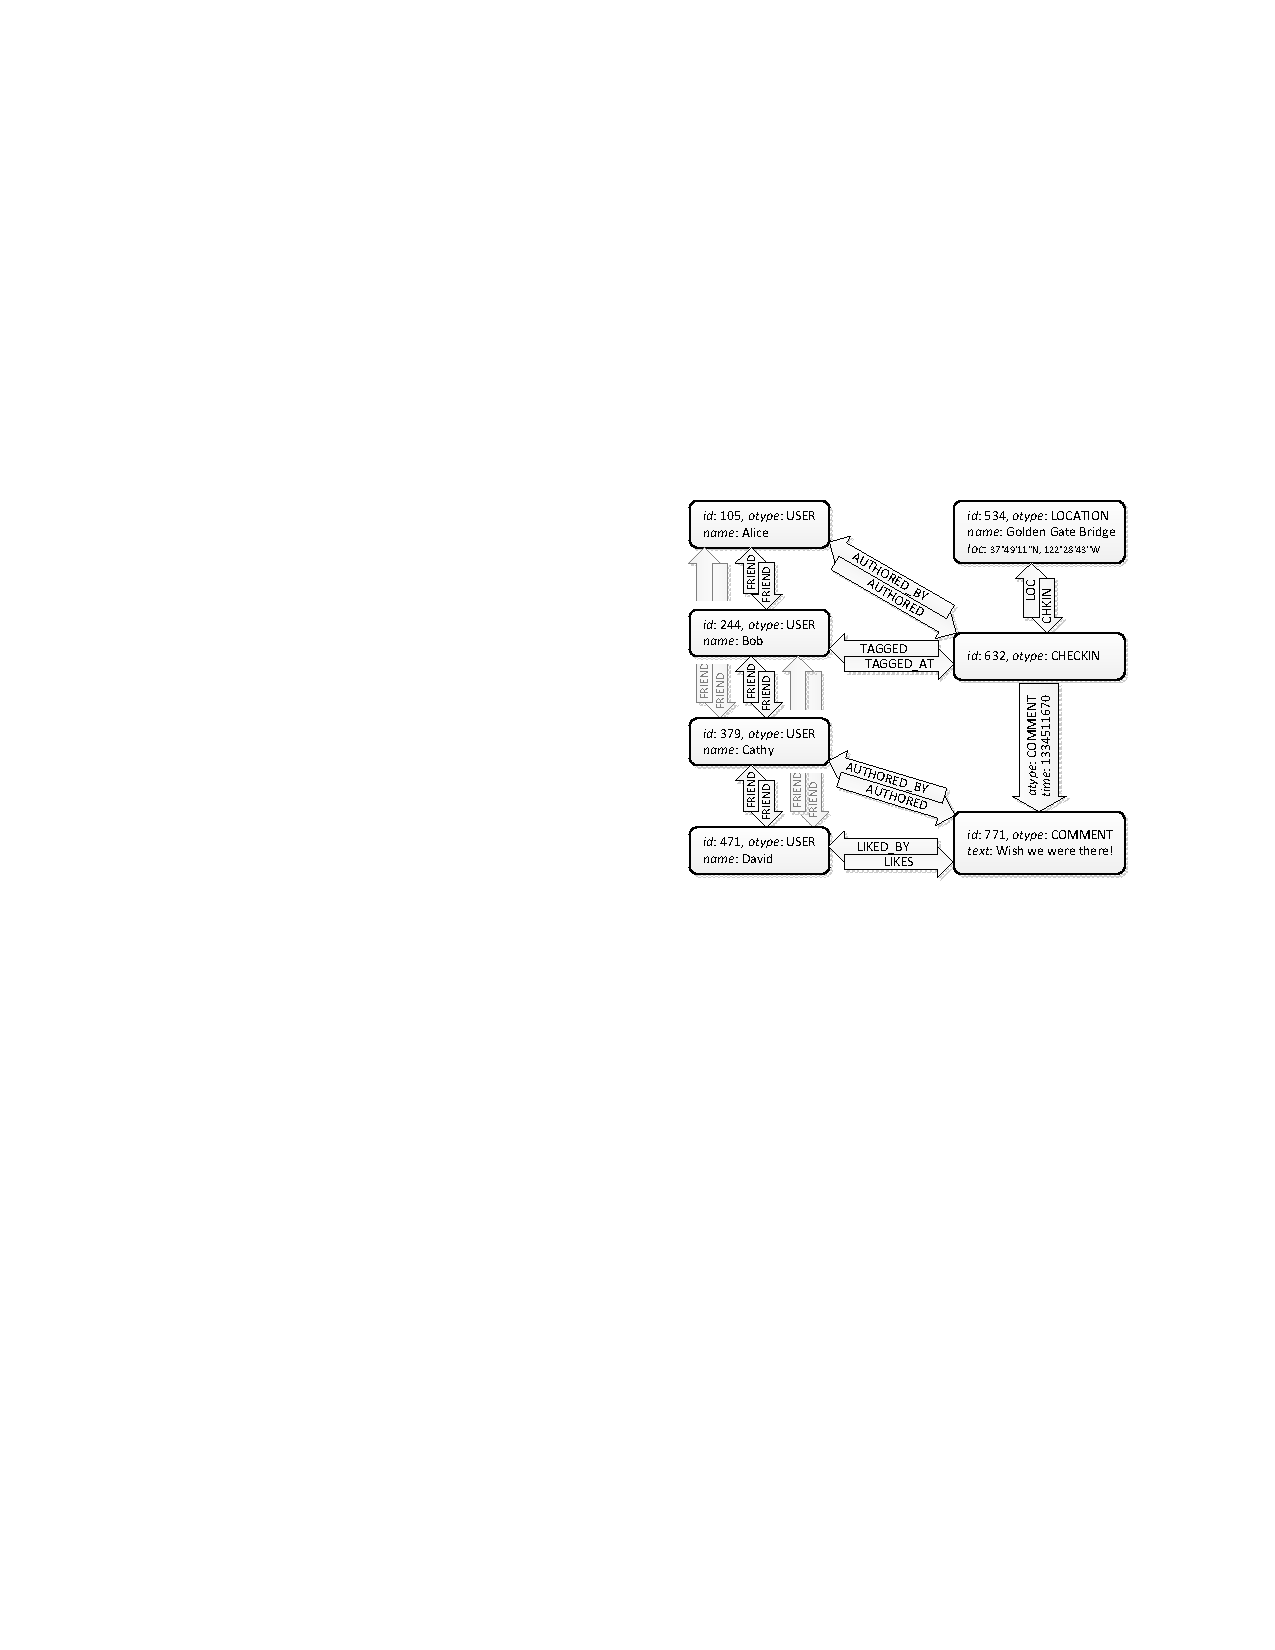
\includegraphics[width=0.6\textwidth]{figs/social2}		
 	\end{center}
\end{frame}

\begin{frame}[fragile]
\frametitle{Objects}
   
\begin{itemize}
	\item Typed nodes (type is denoted by \verb|otype|)
	\item Identified by 64-bit integers. (unique) 
	\item Contains data in the form of key-value pairs.
	\item Models users and repeatable actions (eg comments).
\end{itemize}
 


\end{frame}


\begin{frame}
\frametitle{Associations}
    


\end{frame}
%!TEX root = presentazionelancia.tex
\section{Architecture}
\begin{frame}[t]
\frametitle{Architecture}
    \onslide<1>Before Tao
    \begin{center}
    	\includegraphics<1>[width=0.6\textwidth]{figs/before_tao.jpg}
    \end{center}
	\onslide<2>After Tao
	\begin{center}
    	\includegraphics<2>[width=0.6\textwidth]{figs/tao_arch.jpeg}
    \end{center}
\end{frame}

\begin{frame}[fragile]
\frametitle{Storage Layer}
\begin{itemize}
	\item Object and Associations are stored in MySql (before \& with TAO)	
	\item TAO API is mapped to a small set of SQL queries
	\item A single MySql server can't handle TAO volumes of data
	\begin{itemize}
		\item We divide data into logical \emph{shards}
		\item \emph{shards} are mapped to db 
		\item different servers are responsible for multiple shards
		\item mapping is adjusted for load balancing
	\end{itemize}
	\item Object are bounded to a \emph{shard} for their entire lifetime
	\item Associations are stored in the \emph{shard} of its \verb!id1!
\end{itemize}
\end{frame}

\begin{frame}[c]\frametitle{Cache Layer}
    TAO cache 
    \begin{itemize}
    	\item contains: Objects, Associations, Associations counts
    	\item implement the complete API for clients
    	\item handles all the communication with storage layer
    	\item it's filled on demand end evict the least recently used items
    	\item Understand the semantic of their contents
    \end{itemize}

    It consists of multiple servers forming a \emph{tier}
    \begin{itemize}
    	\item Request are forwarded to correct server by a \emph{sharding} scheme as dbs
    	\item For cache miss and write request, the server contacts other caches or db
    \end{itemize}
    
\end{frame}
\begin{frame}[c]\frametitle{Yet Another caching layer}
	\onslide<1->\textbf{Problem: }A single caching layer divided into a \emph{tier} is susceptible to \emph{hot spot}

	\onslide<2->\textbf{Solution: }Split the caching layer in two levels
	\onslide<2->\begin{itemize}
		\item A \emph{Leader} tier
		\item Multiple \emph{Followers}	tiers
	\end{itemize}
\end{frame}

\begin{frame}[c]\frametitle{Leaders \& Followers}
    


\end{frame}


%!TEX root = presentazionelancia.tex
\section{Implementation}
\begin{frame}
\frametitle{Implementation}
To achieve performance and storage efficiency Fb have implemented some optimizations to servers and DBMS's. 
\end{frame}

\begin{frame}[c]\frametitle{Caching Servers}
\begin{itemize}
	\item Memory is partitioned into arenas by association type
	\begin{itemize}
		\item This mitigates the issues of poorly behaved association types
		\item They can also change the lifetime for important associations
	\end{itemize}
	\item Small items with fixed size have a lot of pointer overhead
	\begin{itemize}
		\item They use a directly mapped 8-way LRU cache
		\item Used for association counts
	\end{itemize}
\end{itemize}    
\end{frame}

\begin{frame}[c]\frametitle{MySql Mapping}
    We divided the space of objects and associations into \emph{shards}. Each \emph{shard}:
    \begin{itemize}
    	\item is assigned to a logical DB
    	\item a
    \end{itemize}


\end{frame}
%!TEX root = presentazionelancia.tex
\section{Consistency \& Failures}
\begin{frame}[t]\frametitle{Consistency}
    


\end{frame}
%!TEX root = presentazionelancia.tex
\section{Workload \& Performance}
\begin{frame}[t]\frametitle{title}
    


\end{frame}

\setbeamercolor{background canvas}{bg=matblue}
\setbeamercolor{normal text}{fg=white}
\begin{frame}[plain, b]
\centering
\huge \textcolor{white}{Thank You}
\normalsize

\vspace*{\fill}

 \begin{beamercolorbox}[wd=\paperwidth]{section in head/foot}
 \centering
Facebook Tao - A Distributed Data Store for the Social Graph
\vskip10pt
\end{beamercolorbox}
 \end{frame}

\end{document}
